\documentclass[main.tex,fontsize=12pt,paper=a4,paper=landscape,DIV=calc,]{scrartcl}
% Document
\usepackage[T1]{fontenc}
\usepackage[utf8]{inputenc}
\usepackage[dvipsnames]{xcolor}
\usepackage[nswissgerman,english]{babel} 
\usepackage{hyperref}
\renewcommand{\familydefault}{\sfdefault}

% Format
\usepackage[top=5mm,bottom=5mm,left=5mm,right=5mm]{geometry}
%\setlength{\headheight}{\baselineskip}
%\setlength{\headsep}{0mm}

%\usepackage{scrlayer-scrpage}
%\clearpairofpagestyles
%\chead{{\bfseries\TITLE, \AUTHOR, \pagename~\thepage}}

%\addtokomafont{pagehead}{\upshape}

\usepackage{multicol}
\setlength{\columnsep}{2mm}
\setlength{\columnseprule}{0.1pt}

% Math
\usepackage{amsmath}
\usepackage{amssymb}
\usepackage{amsfonts}

% Code
\usepackage{fancyvrb, etoolbox, listings, xcolor}
%\usemintedstyle{bw}

%\newminted[shell]{bash}{
%fontsize=\footnotesize,
%fontfamily=tt,
%breaklines=true,
%frame=single,
%framerule=0.1pt,
%framesep=2mm,
%tabsize=2
%}
%\newminted{css}{
%breaklines=true,
%tabsize=4,
%autogobble=true,
%escapeinside=||,
%stripall=true,
%stripnl=true,
%}

    \definecolor{lightgray}{rgb}{0.95, 0.95, 0.95}
    \definecolor{darkgray}{rgb}{0.4, 0.4, 0.4}
    \definecolor{purple}{rgb}{0.65, 0.12, 0.82}
    \definecolor{ocherCode}{rgb}{1, 0.5, 0} % #FF7F00 -> rgb(239, 169, 0)
    \definecolor{blueCode}{rgb}{0, 0, 0.93} % #0000EE -> rgb(0, 0, 238)
    \definecolor{greenCode}{rgb}{0, 0.6, 0} % #009900 -> rgb(0, 153, 0)
    \definecolor{teal}{rgb}{0.0, 0.5, 0.5}

\lstdefinestyle{code}{
    identifierstyle=\color{black},
    keywordstyle=\color{blue}\bfseries\small,
    ndkeywordstyle=\color{greenCode}\bfseries\small,
    stringstyle=\color{ocherCode}\ttfamily\small,
    commentstyle=\color{teal}\ttfamily\textit\small,
    basicstyle=\ttfamily\small,
    breakatwhitespace=false,         
    breaklines=true,                 
    captionpos=b,                    
    keepspaces=true,                 
    showspaces=false,                
    showstringspaces=false,
    showtabs=false,                  
    tabsize=2,
    belowskip=-5pt
}



% Images
\usepackage{graphicx}
\newcommand{\pic}{\includegraphics[scale=0.3]}
\graphicspath{{Screenshots/}{../Screenshots}}
\makeatletter
\def\pictext#1#2{%
    \@ifnextchar[{%
    \pictext@iiiii{#1}{#2}%
    }{%
      \pictext@iiiii{#1}{#2}[0.5,0.4,0.3]% Default is 5
    }%
}
\def\pictext@iiiii#1#2[#3,#4,#5]{\begin{minipage}{#3\textwidth}\includegraphics[scale=#4]{#1}\end{minipage}\begin{minipage}{#5\textwidth}#2\end{minipage}}
\def\minipg#1#2{%
    \@ifnextchar[{%
    \minipg@iiii{#1}{#2}%
    }{%
      \minipg@iiii{#1}{#2}[0.3,0.6]% Default is 5
    }%
}
\def\minipg@iiii#1#2[#3,#4]{\vspace{0.8mm}\begin{minipage}{#3\textwidth}#1\end{minipage}\begin{minipage}{#4\textwidth}#2\end{minipage}{\vspace{0.8mm}}}
\makeatother

%\newenvironment{minty}[2]% environment name
%{% begin code
%  \begin{minipage}{#1}
%  \begin{minted}{#2}
%}%
%{% end code
%  \end{minted}
%  \end{minipage}
%  \end{minty}\ignorespacesafterend
%} 

% Smaller Lists
\usepackage{enumitem}
\setlist[itemize,enumerate]{leftmargin=3mm, labelindent=0mm, labelwidth=1mm, labelsep=1mm, nosep}
\setlist[description]{leftmargin=0mm, nosep}
\setlength{\parindent}{0cm}

% Smaller Titles
\usepackage[explicit]{titlesec}

%% Color Boxes
\newcommand{\sectioncolor}[1]{\colorbox{black!60}{\parbox{0.97\linewidth}{\color{white}#1}}}
\newcommand{\subsectioncolor}[1]{\colorbox{black!50}{\parbox{0.97\linewidth}{\color{white}#1}}}
\newcommand{\subsubsectioncolor}[1]{\colorbox{black!40}{\parbox{0.97\linewidth}{\color{white}#1}}}
\newcommand{\paragraphcolor}[1]{\colorbox{black!30}{\parbox{0.97\linewidth}{\color{white}#1}}}
\newcommand{\subparagraphcolor}[1]{\colorbox{black!20}{\parbox{0.97\linewidth}{\color{white}#1}}}

%% Title Format
\titleformat{\section}{\vspace{0.3mm}\bfseries}{}{0mm}{\sectioncolor{\thesection~#1}}[{\vspace{0.3mm}}]
\titleformat{\subsection}{\vspace{0.3mm}\bfseries}{}{0mm}{\subsectioncolor{\thesubsection~#1}}[{\vspace{0.3mm}}]
\titleformat{\subsubsection}{\vspace{0.3mm}\bfseries}{}{0mm}{\subsubsectioncolor{\thesubsubsection~#1}}[{\vspace{0.3mm}}]
\titleformat{\paragraph}{\vspace{0.3mm}\bfseries}{}{0mm}{\paragraphcolor{\theparagraph~#1}}[{\vspace{0.3mm}}]
\titleformat{\subparagraph}{\vspace{0.3mm}\bfseries}{}{0mm}{\subparagraphcolor{\thesubparagraph~#1}}[{\vspace{0.3mm}}]

%% Title Spacing
\titlespacing{\section}{0mm}{0mm}{0mm}
\titlespacing{\subsection}{0mm}{0mm}{0mm}
\titlespacing{\subsubsection}{0mm}{0mm}{0mm}
\titlespacing{\paragraph}{0mm}{0mm}{0mm}
\titlespacing{\subparagraph}{0mm}{0mm}{0mm}

%% format cells
\usepackage[document]{ragged2e}
\usepackage{array, makecell}
\renewcommand{\arraystretch}{2}
\newcommand{\mc}{\makecell[{{m{1\linewidth}}}]}




\lstset{
    language=[Sharp]C,
    style=code,
}

\begin{document}
\begin{multicols*}{4}

\section{vector geometry}
Point: P (5,2)\newline
vector: \(\vec{v} \left(\dfrac{5}{2}\right)\) \footnotesize not used here to save space
\normalsize

\subsection{Translation | linear}
P + \(\vec{v} \) = (1,2,3) + (4,5,6) = (5,6,9) 

\subsection{Scaling | linear}
P * s = (s * 1, s * 2, s * 3)

\subsection{Rotation | NOT linear}
\(R_\theta \left(\dfrac{x}{0}\right) = \left(\dfrac{cos \theta}{sin \theta} x\right)\)\newline
\(R_\theta \left(\dfrac{0}{y}\right) = \left(\dfrac{-sin \theta}{cos \theta} y\right)\)\newline
\(R_\theta \left(\dfrac{x}{y}\right) = \left(\dfrac{x * cos \theta - y * sin \theta}{x * sin \theta + y * cos \theta} x\right)\)

\subsection{Multiplication of Vectors}
\textbf{Multiplication of vectors is not communitative!}\newline
\(\left[\begin{smallmatrix}\textcolor{blue}{x_{11} \, x_{12} \, x_{13}} \\ x_{21} \, x_{22} \, x_{23} \end{smallmatrix}\right] *
\left[\begin{smallmatrix} \textcolor{green}{y_{11}} \, y_{12} \\ \textcolor{green}{y_{21}} \, y_{22} \\ 
\textcolor{green}{y_{31}} \, y_{32}\end{smallmatrix}\right] =
\left[\begin{smallmatrix} \textcolor{red}{c_{11}} \, c_{12} \\ c_{21} \, c_{22} \end{smallmatrix}\right]\)\newline
\textbf{\textcolor{red}{!! each row * each column !!}}\newline
\textbf{This also means that the row of the first matrix needs to be as long as the column of the second matrix!}\\

\subsection{Matrix Transpose}
\(\left[\begin{smallmatrix} 1  5 \\ 6  7 \end{smallmatrix}\right]^T == \left[ \begin{smallmatrix} 1  6 \\ 5  7 \end{smallmatrix}\right]\)\newline
\textcolor{purple}{Just swap row and columns}

\subsection{Inverse of a Matrix}
\(A^{-1}A = I\)\newline

\includegraphics[scale=0.2]{2022-10-05-05:07:54.png}

\subsection{Linear Dependence}
if the addition of 2 vectors with a scalar of NOT 0 is not the null-vector, then they are linearly \textbf{independent}.\newline
They are also linearly independent if \textbf{the determinant is NOT 0, or the gauss algorithm ends in unitmatrix}.

\subsection{Length of a vector}
\textcolor{purple}{\( |\vec{v}| = \sqrt{x^2 + y^2 + z^2} \)}

\subsection{Dotproduct}
\textbf{\textcolor{red}{\( \vec{a} * \vec{b} = |\vec{a}| * |\vec{b}| * cos(\alpha) \)}}\newline
returns 0 when angle is 90

\subsection{Crossproduct}
\textbf{\textcolor{red}{\( \vec{a} \text{ x } \vec{b} = |\vec{a}| * |\vec{b}| * sin(\alpha) * n\)}}\newline
This is usually used to get the unit vector of the resulting vector, or to\newline
calculate the area of a parallelogram\newline
\(\alpha\) = angle between the vector \(\vec{a}\) and \(\vec{b}\)\newline
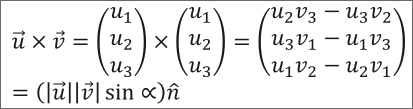
\includegraphics[scale=0.4]{2022-12-27:07:39:36.png}

\subsection{Coordinate systems and spaces}
right handed: positive x to right\newline
left handed: positive x to left\newline
\textcolor{orange}{Local: world without transforms}\newline
\textcolor{orange}{World:} actual 3D representation \newline
Coord: engine defined: ex right handed\newline 
\textcolor{orange}{View:} view transformation for 2D \newline
Coord: engine, 180 rotated\newline
\textcolor{orange}{Clip:} creates 3D illusion\newline
\textcolor{orange}{Screen:} endresult for the human\newline
Coord: without near-far axis (z)

\section{Basics}
\subsection{2D Projection}
camera: (\(e_y, e_z\)), P: (y,z)\newline
\textcolor{purple}{\(\dfrac{c = e_y z - e_z y}{z - e_z}\)}
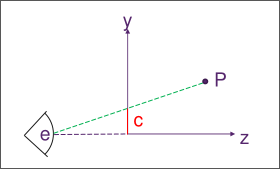
\includegraphics[scale=0.3]{2022-09-21-03:39:39.png}\newline
For a 3D projection you just repeat these steps for each point.\newline
Note, 2D is usually done with \textcolor{red}{\textbf{homogenous coordinates}}, which are just 3D coordinates with a fixed z axis, eg. 1

\subsection{Bresenham Line Algorithm}
\textcolor{purple}{\(y = \dfrac{\delta y}{\delta x}x + c = mx + c\) ==> \(m = \dfrac{\delta y}{\delta x}\)}\newline
\(x = x_0 + \delta x\) \(y = y_0 + m\delta x\) \newline \(\delta x = x - x_0\) \(\delta y = y - y_0 \)

\section{OpenGL}
 \textcolor{purple}{State Machine, Context with ID, \newline Method based, Originally for c++}

\subsection{Meshes}
\textcolor{purple}{Points(x,y,z), Edges, Faces(areas), consisting of triangles}
Vertices can either be indexed, or non-indexed.\newline
\textcolor{orange}{non-indexed vertices will write each point of each triangle, meaning you will have duplicates, indexed vertices will not write each point twice.}\newline
\begin{lstlisting}
// snipped getVertices
for(int j=0; j < sect; j++) {
vert[i++] = Cos(angle);
vert[i++] = Sin(angle);
vert[i++] = 0;
angle += deltaAngle; }
// snipped getTriangles
for(int j=0; j < sect; j++) {
tria[i++] = 0;
tria[i++] = 1 + j;
tria[i++] = 1+(j+1) % sect);}
\end{lstlisting}

\subsection{Perspective Projection}
Similar to 2D projection. \newline
\textcolor{orange}{View Frustum}: \newline
\textbf{fov(y), aspectratio, near and far plane}\newline
\textcolor{OliveGreen}{If the fov is small, then shapes appear big, if the fov is big, the shapes appear small}

\subsection{Orthographic Projection / Parallel Projection}
\textcolor{purple}{normalized coordinates (between -1 and 1)}\newline
\textbf{No Z dimension!}

\section{GPU Pipeline}
\begin{itemize}
\item \textcolor{purple}{Vertex Processor} Programmable\newline
  Turns raw vertices into primitives
\item \textcolor{purple}{Rasterizer} primitives into fragments
\item \textcolor{purple}{Fragment Processor} Programmable \newline
  processes fragments -> ex. color
\item \textcolor{purple}{Output Merging} Fragments to pixels
\end{itemize}
Note a shader would program both the vertex and the fragment processor!

\subsection{Double Buffering}
This seperates the writing and reading of frames, making sure there are no artifacts when displaying the frame, see tearing!

\section{Lighting}
\subsection{Subtractive Light (CMYK) on Remission}
\textcolor{purple}{Start with white, then remove colors}\newline
When an object remits light, it will only show colors that are both in the light AND on the object itself:\newline
\textcolor{purple}{\(C = C_L^T * C_0\)}\newline
\(C_0\) is the original color\newline
\textcolor{red}{The base Cyan, Magenta, Yellow are stored in RGB vectors!}

\subsection{Additive Lighting}
\textcolor{purple}{Start with black, then add colors}\newline
\textcolor{purple}{\(C = 1 - (1 - C_{L1} )^T (1 - C_{L2} )\)}

\subsection{Ambient Lighting}
\textcolor{purple}{Diffuse Lighting from all direcitons, Remission in all directions}

\end{multicols*}
\end{document}
